% !TeX spellcheck = de_DE
\documentclass[12pt]{article}
\usepackage[utf8]{inputenc}
\usepackage{geometry}
\usepackage{svg}
\usepackage{float}
\usepackage{caption}
\usepackage{amsmath,amsthm,amsfonts,amssymb,amscd}
\usepackage{fancyhdr}
\usepackage{titlesec}
\usepackage{hyperref}
\usepackage{listings}
\usepackage[skip=3pt]{parskip}
\usepackage[ngerman]{babel}
\pagestyle{empty}
\titleformat*{\section}{\large\bfseries}
\titleformat*{\subsection}{\bfseries}

%
\geometry{
	a4paper,
	total={170mm,240mm},
	left=20mm,
	top=30mm,
}

\date{}
%Bitte ausfüllen
\newcommand\course{Software Architectures for Enterprises}
\newcommand\hwnumber{\large Portfolio 2}
\newcommand\Name{Fabian Sponholz}
\newcommand\Neptun{1561546}

%Matheinheiten
\newcommand\m{\:\textrm{m}}
\newcommand\M{\:\Big[\textrm{m}\Big]}
\newcommand\mm{\:\textrm{mm}}
\newcommand\MM{\:\Big[\textrm{mm}\Big]}
\newcommand\un{\underline}
\newcommand\s{\:\textrm{s}}
\newcommand\bS{\:\Big[\textrm{S}\Big]}
\newcommand\ms{\:\frac{\textrm{m}}{\textrm{s}}}
\newcommand\MS{\:\Big[\frac{\textrm{m}}{\textrm{s}}\Big]}
\newcommand\mss{\:\frac{\textrm{m}}{\textrm{s}^2}}
\newcommand\MSS{\:\Big[\frac{\textrm{m}}{\textrm{s}^2}\Big]}

%Trennlinie
\newcommand\separator{\rule{\linewidth}{0.5pt}}

%Bitte nicht einstellen
\renewcommand{\figurename}{Abbildung}
\renewcommand{\tablename}{Tabelle}
\pagestyle{fancyplain}
\headheight 35pt
\lhead{\Name\\\Neptun}
\chead{\textbf{ \hwnumber}}
\rhead{\course \\ \today}
\lfoot{}
\cfoot{}
\rfoot{\small\thepage}
\headsep 1.5em

\begin{document}
	
\section*{Aufgabe 1 - Modellierung}
\subsection*{Zu erwartendes Lastaufkommen}
Bei der Berechnung des erwarteten Lastaufkommens in der Vorweihnachtszeit gehen wir vereinfacht davon aus, dass es auf der Welt etwa 5 Milliarden Kinder und kindgebliebene Erwachsene gibt, die ihre Wunschliste an Santa Claus übermitteln möchten.
Außerdem gehen wir davon aus, dass all diese Einsendungen innerhalb von 90 Tagen (im letzten Quartal) eingehen und jede Person nur \emph{einen} Wunschzettel, wenn auch mit mehreren Wünschen, einsendet.

Dabei wurde vereinfachend die Annahme gemacht, dass die gesamte Menschheit den Weihnachtsmann als religions- und kulturunabhängige Instanz respektiert und eine fristgerechte Lieferung der Geschenke an dem sich historisch in einer seit Jahrtausenden fortlaufenden Studie als am günstigsten herausgestellten Liefertermin (dem 24.12.) gewohnt ist.
Maßgeblich bei der Berechnung des Liefertermins ist das zu diesem Zeitpunkt vorliegende Gleichgewicht zwischen Gemütlichkeit des Abends (nimmt mit Fortschreiten des Winters zu) und Wahrscheinlichkeit einer schneesturmfreien Nacht (nimmt mit Fortschreiten des Winters ab).
Dabei wird entgegen der Realität davon ausgegangen, dass der Jahreszeitenzyklus überall auf der Erde synchron verläuft.

Wie dem auch sei, das System durchläuft jedes Jahr drei Phasen, die je ein wachsendes Anfrageaufkommen im \emph{XMasWishes}-System erwarten lassen:

\begin{itemize}
	\item \textbf{Phase 1: Wunschlisten-Einsammel-Phase} - 90 Tage vor dem Stichtag wird das System auf öffentlich geschaltet und ist bereit für eingehende Wunschlisten. Dabei wird innerhalb dieser Zeit etwa 5 Milliarden mal schreibend auf das System zugegriffen. Die Anfragefrequenz in Hertz berechnet sich wie folgt: 
	$$freq_{collection} = 5000000000 \div (90 \cdot 24 \cdot 60 \cdot 60) hz \approx 650 hz $$
	
	\item \textbf{Phase 2: Produktionsphase} - In den letzten 30 Tagen vor dem Stichtag produzieren die Elfen alle Geschenke. Hierbei fragt jeder Elf aus dem System einen Wunsch ab, der noch nicht bearbeitet wurde, um diesen dann umzusetzen. Der Wunsch wird dann auf \emph{In Bearbeitung} gesetzt. Hier wird jeder Wunsch genau ein mal abgefragt. Bei durchschnittlich 3 Wünschen pro Wunschzettel ergibt sich das Anfrageaufkommen wie folgt:
	$$freq_{production} = 3 \cdot 5000000000 \div (30 \cdot 24 \cdot 60 \cdot 60) hz \approx 5800 hz$$
	
	\item \textbf{Phase 3:Auslieferungsphase} - Am Stichtag lädt der Weihnachtsmann alle Geschenke auf seinen Schlitten und setzt den Zustand aller Geschenke von \emph{In Bearbeitung} auf \emph{In Zustellung}. Dies ist mit einem einzelnen Aufruf möglich.
	Danach ruft er während der Auslieferung jede Wunschliste noch einmal ab, um in jedem Haus die passenden Geschenke abzuliefern.
	Wem unrealistisch erscheint, dass der Weihnachtsmann alle Geschenke selbst ausliefert, dem sei gesagt, dass der Weihnachtsmann sich mithilfe modernster Quantentechnologie stets in einer Superposition befindet und somit an mehreren Orten gleichzeitig sein kann.
	Es wird also innerhalb eines Tages jede Wunschliste einmal in einem Aufruf abgerufen und die entsprechenden Geschenke danach als ausgeliefert markiert.
	Das Anfrageaufkommen ergibt sich dann wie folgt:
	$$freq_{delivery} = 2 \cdot 5000000000 \div (1 \cdot 24 \cdot 60 \cdot 60) hz \approx120000 hz$$
	
\end{itemize}

\subsection*{Modellierung einer skalierbaren Architektur für XMasWishes}
Folgender Ansatz wird in diesem Projekt umgesetzt:

\begin{itemize}
	\item \textbf{Backend:} Horizontal skalierbare, verteilte Datenbank.
	\item \textbf{Business-Logik:} Stateless Service, der die Schnittstelle zwischen Nutzer und Datenbank herstellt. Kann beliebig oft repliziert werden.
	\item \textbf{Load-Balancer} Wird zwischen Frontend und Business-Logik geschaltet, um die Last gleichmäßig auf die Services zu verteilen.
	\item \textbf{Frontend} Web-Applikation im Browser des Nutzers, ggf. auf dem gleichen Server wie die Business-Logik gehostet.
\end{itemize}

Ein Authentifizierungsservice wie OAuth wird nicht implementiert, da der Nordpol bereits über eine quantenbasierte Firewall verfügt, die sicherstellt, dass jeder nur auf das zugreifen kann, was er benötigt.

\section*{Aufgabe 2 - Konkretisierung}

\begin{figure}[H]
	\centering
	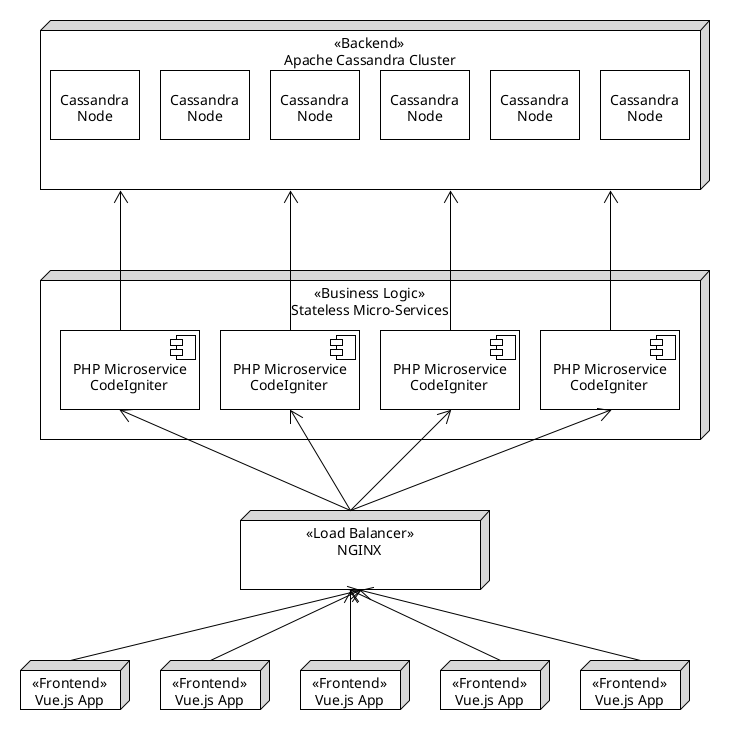
\includegraphics[width=0.8\textwidth]{./img/architecture}
	\caption{Architektur des Systems}
\end{figure}

Ich habe mich bei der Implementierung für folgende Technologien entschieden:
\begin{itemize}
	\item \textbf{Backend:} Als Backend-Datenbank habe ich mich für \textbf{Apache Cassandra} entschieden. Dabei handelt es sich um eine horizontal skalierbare, verteilte NoSQL-Datenbank, die eine relationale Datenbank simuliert und mit einer SQL-Ähnlichen Sprache angesprochen wird.
	Sie skaliert in Performance und Speicherkapazität linear mit der Anzahl der Knoten und ist somit ideal für große Datenmengen und großes Transaktionsaufkommen geeignet.
	Mithilfe von Hashing wird bereits durch den Datenbank-Driver des Clients (in diesem Fall der Geschäftslogik) festgestellt, auf welchem Datenbank-Node eine Anfrage am schnellsten bearbeitet werden kann.
	So wird die Last optimal auf das Cluster verteilt.
	\item \textbf{Business-Logik:} Bei der Business-Logik setze ich auf \textbf{RESTful Microservices}, bzw. in diesem Fall nur einen WishlistService, der die Wunschlisten und Wünsche verwaltet.
	Weitere Microservices wie eine Nutzerverwaltung und einen Authentifizierungs-Service spare ich mir an dieser Stelle, könnten aber einfach hinzugefügt werden.
	Diese Services sind stateless (speichern keine Sitzungsdaten), und können daher einfach repliziert werden.
	Als Technologie habe ich mich für \textbf{PHP} mit dem Framework \textbf{CodeIgniter} entschieden.
	Vorteil daran ist, dass der Service auf einem normalen Apache-Webserver läuft, der sehr leichtgewichtig ist.
	CodeIgniter ist ebenfalls ein Framework, dass sehr auf Performance und Leichtgewicht optimiert ist, und nur die nötigsten Funktionen zur Verfügung stellt, so zum Beispiel eingebautes Routing, Separation nach dem MVC-Modell, diverse eingebaute Datenbank-Treiber sowie einige essenzielle Sicherheits-Features.
	Durch das Hosting auf einem Apache-Server und die Verwendung von CodeIgniter könnte außerdem die Verteilung von Frontend-Websites auch über diesen Service realisiert werden.
	\item \textbf{Load-Balancer:} Um die Last gleichmäßig auf die Instanzen des WishlistService zu verteilen, wird \textbf{NGINX} als Load-Balancer verwendet. NGINX ist ein hochperformanter Webserver, Reverse-Proxy und Load-Balancer, der in diesem Fall die Anfragen nach dem Round-Robin-Prinzip auf die vorhandenen Services verteilt. Er erkennt außerdem Ausfälle einzelner Service-Instanzen und leitet Anfragen ggf. um.
	\item \textbf{Frontend:} Das Frontend wird als \textbf{Vue.js Single-Page-Applikation} realisiert. Dadurch wird die gesamte App mit dem ersten Aufruf des Web-Links geladen und dann lokal beim Nutzer gecached.
	So wird die Last des Webservers reduziert.
	Um die Last des Webservers weiter zu reduzieren, kann auch dieser repliziert und hinter einen Load Balancer geschaltet werden.
	Außerdem wäre es möglich, Bilder, CSS- und Javascript-Dateien über ein \emph{Content Delivery Network (CDN)} bereitzustellen, um so weiter die Last des Webservers zu reduzieren. Dieser müsste dann nur noch eine wenige Zeilen lange HTML-Datei ausliefern. 
\end{itemize}

\section*{Aufgabe 3 - Prototyp}
Um ein verteiltes System zu simulieren, verwende ich \textbf{Docker-Compose} zur Verwaltung einiger Docker-Container, die die entsprechenden Maschinen in der Architektur emulieren.
So ist es auch möglich, die Lösung schnell und einfach auf einem anderen Rechner laufen zu lassen.

Bei der Implementierung habe ich einen Back-to-Front-Ansatz verfolgt.
Ich habe also damit begonnen, die Datenbank einzurichten, dann die Microservices erstellt, den Load-Balancer konfiguriert und zuletzt die Frontend-Applikation gebaut.

Für die Datenbank habe ich ein Cassandra-Cluster mit drei Knoten erstellt. Sobald das Cluster erfolgreich hochgefahren ist, startet ein weiterer Cassandra-Container, der mithilfe von \texttt{cqlsh} eine CQL-Datei auf der Datenbank ausführt, um den Keyspace und die benötigten Tabellen einzurichten. Dies ist nur beim ersten Hochfahren des Clusters relevant, da die Daten in den Containern der Nodes persistent gespeichert sind.


	
\end{document}